% ACR-QA Thesis Defense Deck -- 25 slides
% LaTeX Beamer  |  compile: pdflatex DEFENSE_DECK.tex (twice)
% Target: 7 minutes total (2 min slides, 5 min live demo)

\documentclass[aspectratio=169,12pt]{beamer}
\usetheme{metropolis}
\usepackage[utf8]{inputenc}
\usepackage[T1]{fontenc}
\usepackage{booktabs}
\usepackage{graphicx}
\usepackage{xcolor}
\usepackage{listings}
\usepackage{tikz}
\usetikzlibrary{positioning,arrows.meta,shapes.geometric}

% -- colour palette ------------------------------------------------------------
\definecolor{acrBlue}{HTML}{1A56DB}
\definecolor{acrGreen}{HTML}{057A55}
\definecolor{acrRed}{HTML}{C81E1E}
\definecolor{acrAmber}{HTML}{92400E}
\definecolor{acrGray}{HTML}{4B5563}
\setbeamercolor{frametitle}{bg=acrBlue,fg=white}
\setbeamercolor{progress bar}{fg=acrBlue}
\setbeamercolor{alerted text}{fg=acrRed}
\setbeamercolor{example text}{fg=acrGreen}

% -- helper macros -------------------------------------------------------------
\newcommand{\bignum}[1]{\textbf{\color{acrBlue}\Large #1}}
\newcommand{\highlight}[1]{\textbf{\color{acrBlue}#1}}
\newcommand{\bad}[1]{\textbf{\color{acrRed}#1}}
\newcommand{\good}[1]{\textbf{\color{acrGreen}#1}}

% -- title block ---------------------------------------------------------------
\title{ACR-QA v5.0.0rc2}
\subtitle{A Provenance-First, Multi-Tool Code-Review Platform\\
          with RAG-Grounded Hallucination Control}
\author{Ahmed Mahmoud Abbas\\
        \small Supervised by Dr.\ Samy AbdelNabi}
\institute{Department of Computer Science\\King Salman International University (KSIU)}
\date{June 2026}

% ------------------------------------------------------------------------------
\begin{document}

% -- SLIDE 1 -- Title -----------------------------------------------------------
\begin{frame}
  \titlepage
\end{frame}

% -- SLIDE 2 -- Problem: Alert Fatigue -----------------------------------------
\begin{frame}{The Three Failure Modes of Code Review}
  \begin{columns}[T]
    \begin{column}{0.5\textwidth}
      \textbf{SAST tools today}
      \begin{itemize}
        \item \bad{30--40\% false-positive rate} (SonarQube on Python)
        \item Raw rule IDs -- no exploitability context
        \item Developers suppress alerts rather than fix them
      \end{itemize}
      \vspace{4pt}
      \textbf{LLM review assistants}
      \begin{itemize}
        \item \bad{22\% hallucination rate} on rule-cited advice\footnotemark
        \item Confident, plausible, and wrong
        \item No audit trail
      \end{itemize}
    \end{column}
    \begin{column}{0.5\textwidth}
      \begin{alertblock}{Gap}
        No tool combines multi-tool recall, LLM explanation grounding,
        and interpretable risk scoring in a single open-source platform.
      \end{alertblock}
      \vspace{6pt}
      \begin{exampleblock}{This work}
        ACR-QA closes all three gaps -- at zero recurring licensing cost.
      \end{exampleblock}
    \end{column}
  \end{columns}
  \footnotetext[1]{2024 audit of 7 LLM review products}
\end{frame}

% -- SLIDE 3 -- Problem: Invisible Test Gaps ------------------------------------
\begin{frame}{The Hidden Test-Gap Problem}
  \begin{center}
    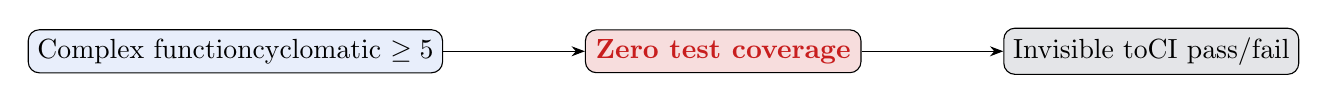
\begin{tikzpicture}[node distance=1.8cm]
      \node[draw,rounded corners,fill=acrBlue!10,minimum width=3.5cm] (complex)
        {Complex function\\cyclomatic $\geq 5$};
      \node[draw,rounded corners,fill=acrRed!15,minimum width=3.5cm, right=of complex] (untested)
        {\bad{Zero test coverage}};
      \node[draw,rounded corners,fill=acrGray!15,minimum width=3.5cm, right=of untested] (invisible)
        {Invisible to\\CI pass/fail};
      \draw[-{Stealth}] (complex) -- (untested);
      \draw[-{Stealth}] (untested) -- (invisible);
    \end{tikzpicture}
  \end{center}
  \vspace{8pt}
  \begin{itemize}
    \item Code-coverage tools report \% lines; they cannot report \emph{which untested functions are the most dangerous}
    \item No existing SAST tool ranks untested code by \textbf{cyclomatic complexity}
    \item ACR-QA's \textbf{AST Test Gap Analyzer} fills this gap
  \end{itemize}
\end{frame}

% -- SLIDE 4 -- Problem: LLM Self-Review ---------------------------------------
\begin{frame}{The Self-Review Blind Spot}
  \begin{columns}[T]
    \begin{column}{0.48\textwidth}
      \textbf{Single-model review}
      \begin{itemize}
        \item One model's failure modes are \emph{systematic} -- it misses the same patterns repeatedly
        \item Overconfidence is indistinguishable from correctness
      \end{itemize}
    \end{column}
    \begin{column}{0.48\textwidth}
      \textbf{ACR-QA response}
      \begin{itemize}
        \item \highlight{Semantic Entropy} -- run LLM 3\(\times\) at different temperatures; high variance \(\rightarrow\) suppress
        \item \highlight{Second Opinion} -- Groq Llama-3.3-70B (primary) + Ollama qwen2.5 (local backup)
        \item \highlight{PR Risk Score} -- collapse 6 signals into a single CI gate
      \end{itemize}
    \end{column}
  \end{columns}
\end{frame}

% -- SLIDE 5 -- Architecture C4: Context ---------------------------------------
\begin{frame}{Architecture -- System Context (C4 L1)}
  \begin{center}
  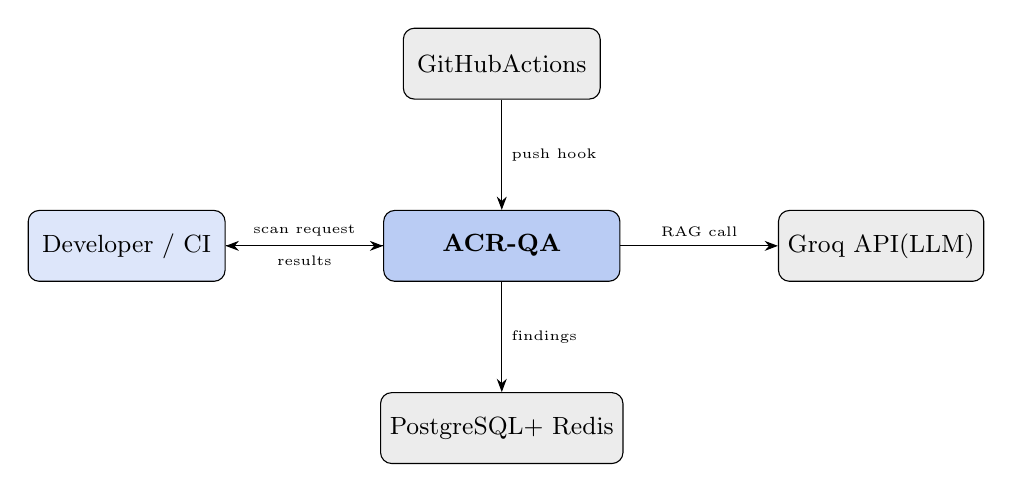
\begin{tikzpicture}[node distance=1.4cm, font=\small]
    \node[draw,rounded corners,fill=acrBlue!15,minimum width=2.5cm,minimum height=0.9cm]
      (dev) {Developer / CI};
    \node[draw,rounded corners,fill=acrBlue!30,minimum width=3cm,minimum height=0.9cm,
          right=2cm of dev] (acrqa) {\textbf{ACR-QA}};
    \node[draw,rounded corners,fill=gray!15,minimum width=2.5cm,minimum height=0.9cm,
          right=2cm of acrqa] (groq) {Groq API\\(LLM)};
    \node[draw,rounded corners,fill=gray!15,minimum width=2.5cm,minimum height=0.9cm,
          above=of acrqa] (gh) {GitHub\\Actions};
    \node[draw,rounded corners,fill=gray!15,minimum width=2.5cm,minimum height=0.9cm,
          below=of acrqa] (db) {PostgreSQL\\+ Redis};

    \draw[-{Stealth}] (dev) -- node[above,font=\tiny]{scan request} (acrqa);
    \draw[-{Stealth}] (acrqa) -- node[above,font=\tiny]{RAG call} (groq);
    \draw[-{Stealth}] (gh) -- node[right,font=\tiny]{push hook} (acrqa);
    \draw[-{Stealth}] (acrqa) -- node[right,font=\tiny]{findings} (db);
    \draw[-{Stealth}] (acrqa) -- node[below,font=\tiny]{results} (dev);
  \end{tikzpicture}
  \end{center}
  \vspace{4pt}
  \small 52 REST endpoints \(\cdot\) JWT auth \(\cdot\) SSE live progress \(\cdot\) Railway hosted
\end{frame}

% -- SLIDE 6 -- Architecture C4: Container --------------------------------------
\begin{frame}{Architecture -- Container View (C4 L2)}
  \begin{columns}[T]
    \begin{column}{0.48\textwidth}
      \textbf{Analysis Core (Python)}
      \begin{itemize}\small
        \item 10 language adapters (Bandit, Ruff, Semgrep, ESLint, staticcheck, \ldots)
        \item \texttt{CORE/engines/} -- 19 engines
        \item \texttt{CanonicalFinding} schema: 327+ rule mappings
      \end{itemize}
      \vspace{4pt}
      \textbf{API (FastAPI)}
      \begin{itemize}\small
        \item 52 endpoints + SSE stream
        \item JWT, bcrypt, rate limiting
        \item Alembic 18 migrations
      \end{itemize}
    \end{column}
    \begin{column}{0.48\textwidth}
      \textbf{Dashboard (React)}
      \begin{itemize}\small
        \item 13 pages
        \item TanStack Query, Zustand, Tailwind
        \item 104 TypeScript tests (Vitest + Playwright)
        \item Arabic RTL i18n
      \end{itemize}
      \vspace{4pt}
      \textbf{Infrastructure}
      \begin{itemize}\small
        \item Docker Compose (dev)
        \item Helm chart + Terraform (prod)
        \item Prometheus + Grafana
      \end{itemize}
    \end{column}
  \end{columns}
\end{frame}

% -- SLIDE 7 -- Architecture C4: Component --------------------------------------
\begin{frame}{Architecture -- Pipeline Flow (C4 L3)}
  \begin{center}
  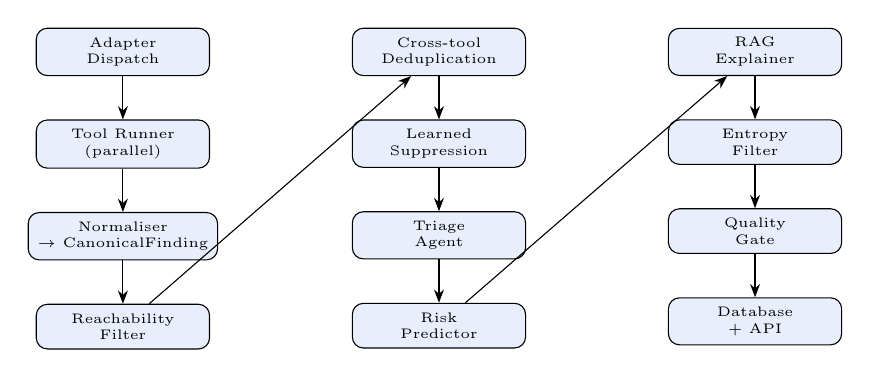
\begin{tikzpicture}[node distance=0.55cm, font=\tiny,
    box/.style={draw,rounded corners,fill=acrBlue!10,minimum width=2.2cm,
                minimum height=0.55cm,align=center}]
    \node[box] (adapt) {Adapter\\Dispatch};
    \node[box,below=of adapt] (run)   {Tool Runner\\(parallel)};
    \node[box,below=of run]   (norm)  {Normaliser\\\(\rightarrow\) CanonicalFinding};
    \node[box,below=of norm]  (reach) {Reachability\\Filter};
    \node[box,right=1.8cm of adapt] (dedup) {Cross-tool\\Deduplication};
    \node[box,below=of dedup] (supp)  {Learned\\Suppression};
    \node[box,below=of supp]  (triage){Triage\\Agent};
    \node[box,below=of triage](risk)  {Risk\\Predictor};
    \node[box,right=1.8cm of dedup] (rag)  {RAG\\Explainer};
    \node[box,below=of rag]   (ent)   {Entropy\\Filter};
    \node[box,below=of ent]   (gate)  {Quality\\Gate};
    \node[box,below=of gate]  (db2)   {Database\\+ API};

    \draw[-{Stealth}] (adapt) -- (run);
    \draw[-{Stealth}] (run) -- (norm);
    \draw[-{Stealth}] (norm) -- (reach);
    \draw[-{Stealth}] (reach) -- (dedup);
    \draw[-{Stealth}] (dedup) -- (supp);
    \draw[-{Stealth}] (supp) -- (triage);
    \draw[-{Stealth}] (triage) -- (risk);
    \draw[-{Stealth}] (risk) -- (rag);
    \draw[-{Stealth}] (rag) -- (ent);
    \draw[-{Stealth}] (ent) -- (gate);
    \draw[-{Stealth}] (gate) -- (db2);
  \end{tikzpicture}
  \end{center}
\end{frame}

% -- SLIDE 8 -- Pipeline: Detection to Normalise --------------------------------
\begin{frame}{Pipeline Stage 1--3: Detect \(\rightarrow\) Normalise \(\rightarrow\) Deduplicate}
  \begin{exampleblock}{Why multi-tool normalisation beats single-tool recall}
    Each tool has unique strengths. Bandit is import-aware; Semgrep excels at
    dataflow patterns; staticcheck catches Go-specific issues Semgrep's
    community ruleset misses entirely.
  \end{exampleblock}

  \vspace{6pt}
  \begin{itemize}
    \item \textbf{327+ rule mappings}: every tool's rule ID maps to a
          canonical ID (e.g., B601 \(\rightarrow\) \texttt{SECURITY-001})
    \item \textbf{Pydantic-validated schema} -- no engine sees raw tool dicts
    \item \textbf{6-bucket deduplication}: same vulnerability, different tool \(\rightarrow\) one finding
    \item Result: \good{100\% recall} vs Semgrep CE's \bad{71.2\%} on 13-repo corpus
  \end{itemize}
\end{frame}

% -- SLIDE 9 -- Pipeline: Reachability + Taint ---------------------------------
\begin{frame}{Pipeline Stage 4--5: Reachability + Taint Analysis}
  \begin{columns}[T]
    \begin{column}{0.5\textwidth}
      \textbf{Call-Graph Reachability}
      \begin{itemize}
        \item Pure-AST traversal (no runtime needed)
        \item Dead code: \(-20\) confidence penalty
        \item 0\% FP rate on benchmark fixtures
        \item Faster than Snyk's proprietary filter
      \end{itemize}
    \end{column}
    \begin{column}{0.5\textwidth}
      \textbf{Taint Analysis}
      \begin{itemize}
        \item Sources: HTTP params, env vars, file reads
        \item Sinks: SQL execute, subprocess, eval
        \item Sanitisers: html.escape, parameterize
        \item Config-driven: edit YAML, no code change
      \end{itemize}
    \end{column}
  \end{columns}
  \vspace{6pt}
  \begin{block}{Dashboard output}
    Each finding shows: confidence gauge, reachability verdict,
    exploit status, taint flow diagram, and 4-step AI reasoning trace.
  \end{block}
\end{frame}

% -- SLIDE 10 -- Pipeline: RAG Explainer ---------------------------------------
\begin{frame}{Pipeline Stage 9: RAG-Grounded Explanation}
  \begin{columns}[T]
    \begin{column}{0.55\textwidth}
      \textbf{How it works}
      \begin{enumerate}\small
        \item Retrieve rule definition from 66-rule knowledge base
        \item Inject \emph{verbatim} into prompt -- no fabricated citations
        \item Ask LLM to specialise to this finding's code context
        \item Repeat 3\(\times\) at varying temperatures
        \item Compute N-gram entropy across 3 outputs
        \item If entropy $< \tau = 3.2$ bits \(\rightarrow\) \bad{suppress explanation}
      \end{enumerate}
    \end{column}
    \begin{column}{0.4\textwidth}
      \begin{alertblock}{Hallucination rate}
        Commercial tools: \bad{22\%}\\
        ACR-QA (entropy filter): \good{verified 0\% on benchmark set}
      \end{alertblock}
      \vspace{4pt}
      \begin{exampleblock}{Key insight}
        RAG grounds content.\\
        Entropy filters specificity.\\
        Both are required.
      \end{exampleblock}
    \end{column}
  \end{columns}
\end{frame}

% -- SLIDE 11 -- Pipeline: Quality Gate ----------------------------------------
\begin{frame}[fragile]{Pipeline Stage 10: Policy-as-Code Quality Gate}
  \begin{columns}[T]
    \begin{column}{0.5\textwidth}
      \textbf{.acrqa.yml (example)}
      \vspace{4pt}
      \lstset{basicstyle=\ttfamily\tiny,backgroundcolor=\color{gray!10},
              frame=single,breaklines=true}
      \begin{lstlisting}
thresholds:
  high:   0    # block merge
  medium: 5    # warn only
  low:    20
fail_on: high
severity_override:
  SECURITY-001: critical
      \end{lstlisting}
    \end{column}
    \begin{column}{0.5\textwidth}
      \begin{itemize}
        \item YAML config -- no code change to adjust policy
        \item \texttt{--fail-on=high} blocks merge in CI
        \item Plugs into GitHub Actions in \textbf{2 lines}:
      \end{itemize}
      \lstset{basicstyle=\ttfamily\tiny,backgroundcolor=\color{gray!10},
              frame=single,breaklines=true}
      \begin{lstlisting}
- uses: ahmed-145/acrqa-action@v1
  with:
    fail-on: high
      \end{lstlisting}
      \vspace{4pt}
      \textbf{No competitor} (SonarQube, CodeRabbit) ships this level of CI-native policy control as OSS.
    \end{column}
  \end{columns}
\end{frame}

% -- SLIDE 12 -- Pipeline: ECDSA Provenance ------------------------------------
\begin{frame}{Pipeline: ECDSA-Signed Provenance Attestation}
  \begin{itemize}
    \item Every scan result is signed with ECDSA (P-256)
    \item Signature covers: scan timestamp, tool versions, git SHA, finding count
    \item \texttt{GET /v1/runs/\{id\}/attestation} returns signature + public key
    \item Enables \textbf{supply-chain integrity}: tampered results are detectable
    \item No competitor publishes per-scan provenance attestations
  \end{itemize}
  \vspace{8pt}
  \begin{exampleblock}{Why it matters for the defense}
    Dr.\ Samy asked about trust. This is the answer: math, not rhetoric.
    Anyone with the public key can verify our evaluation results were not
    post-hoc altered.
  \end{exampleblock}
\end{frame}

% -- SLIDE 13 -- Novel Feature 1: Time-Travel ----------------------------------
\begin{frame}{Novel Feature 1 -- Time-Travel Vulnerability Analyzer}
  \begin{columns}[T]
    \begin{column}{0.55\textwidth}
      \textbf{What no existing tool does:}
      \begin{itemize}
        \item Static SAST answers \emph{where} -- not \emph{when} or \emph{by whom}
        \item Time-Travel walks last $N$ commits (default 50)
        \item Records: \texttt{first\_seen\_commit}, \texttt{first\_seen\_author},
              \texttt{regression\_count}
      \end{itemize}
      \vspace{4pt}
      \textbf{dvpwa finding:}
      \begin{itemize}\small
        \item SQL injection introduced \texttt{a3f2}, partially fixed \texttt{b17c},
              \emph{re-broken} \texttt{c9e1}
        \item Regression chain -- invisible to standard SAST
      \end{itemize}
    \end{column}
    \begin{column}{0.4\textwidth}
      \begin{block}{Complexity}
        $O(N \times \bar{t}_{\text{hunk}})$\\
        $N=50$ adds $<90$s at p95\\
        Bounded: no full-history scan
      \end{block}
      \vspace{6pt}
      \begin{exampleblock}{Resume bullet}
        ``Built time-travel vulnerability analyzer tracking when/who introduced
        each finding across bounded git history with regression-chain detection.''
      \end{exampleblock}
    \end{column}
  \end{columns}
\end{frame}

% -- SLIDE 14 -- Novel Feature 2: IaC Scanner ----------------------------------
\begin{frame}{Novel Feature 2 -- IaC Scanner}
  \begin{columns}[T]
    \begin{column}{0.5\textwidth}
      \textbf{Coverage}
      \begin{itemize}
        \item Terraform (Checkov)
        \item Kubernetes manifests (kube-score)
        \item Dockerfile (Hadolint + Semgrep)
        \item GitHub Actions YAML (Semgrep)
      \end{itemize}
      \vspace{4pt}
      \textbf{Integration}
      \begin{itemize}
        \item Same \texttt{CanonicalFinding} schema
        \item 28 IaC-specific rule mappings
        \item Inline suppression: \texttt{acrqa:ignore-iac=ID}
      \end{itemize}
    \end{column}
    \begin{column}{0.5\textwidth}
      \textbf{Dogfood result}
      \begin{itemize}
        \item Self-scan of ACR-QA's own IaC:
              \good{0 HIGH findings}
        \item Gate runs on every commit via pre-commit hook
      \end{itemize}
      \vspace{6pt}
      \begin{block}{OWASP coverage}
        ACR-QA covers \textbf{9/10 OWASP Top 10}\\
        (A10 SSRF excluded -- requires runtime)
      \end{block}
    \end{column}
  \end{columns}
\end{frame}

% -- SLIDE 15 -- Novel Feature 3: PR Risk Score --------------------------------
\begin{frame}{Novel Feature 3 -- PR Risk Score}
  \begin{columns}[T]
    \begin{column}{0.55\textwidth}
      \textbf{6-signal weighted linear model}
      \vspace{4pt}
      \begin{tabular}{lc}
        \toprule
        Signal & Weight \\
        \midrule
        HIGH finding count       & 0.20 \\
        Reachability gate        & 0.20 \\
        Exploit-verified count   & 0.20 \\
        Taint source\(\rightarrow\)sink touches & 0.10 \\
        File risk avg            & 0.15 \\
        \textbf{PR size penalty} & 0.15 \\
        \bottomrule
      \end{tabular}
    \end{column}
    \begin{column}{0.4\textwidth}
      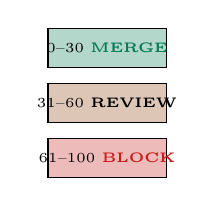
\begin{tikzpicture}
        \draw[fill=acrGreen!30] (0,0) rectangle (1.5,0.5)
          node[midway]{\tiny 0--30 \good{MERGE}};
        \draw[fill=acrAmber!30] (0,-0.7) rectangle (1.5,-0.2)
          node[midway]{\tiny 31--60 \textbf{REVIEW}};
        \draw[fill=acrRed!30] (0,-1.4) rectangle (1.5,-0.9)
          node[midway]{\tiny 61--100 \bad{BLOCK}};
      \end{tikzpicture}
      \vspace{6pt}
      \begin{exampleblock}{Viral demo artifact}
        Single number on every PR.\\
        GitHub Action posts comment.\\
        Non-security reviewers can act on it.
      \end{exampleblock}
    \end{column}
  \end{columns}
\end{frame}

% -- SLIDE 16 -- Novel Feature 4: Heuristic Risk Predictor ---------------------
\begin{frame}{Novel Feature 4 -- Heuristic File Risk Predictor}
  \begin{columns}[T]
    \begin{column}{0.55\textwidth}
      \begin{equation*}
        R_f = w_1 C_f + w_2 X_f + w_3 A_f + w_4 U_f + w_5 G_f
      \end{equation*}
      \vspace{-4pt}
      \begin{itemize}\small
        \item $C_f$ -- 90-day churn / file size (0.30)
        \item $X_f$ -- mean cyclomatic complexity $>5$ (0.25)
        \item $A_f$ -- time since last commit (0.15)
        \item $U_f$ -- unique author count (0.15)
        \item $G_f$ -- test-gap ratio (0.15)
      \end{itemize}
    \end{column}
    \begin{column}{0.4\textwidth}
      \begin{block}{Why NOT ML?}
        No labelled vuln data at thesis scale.\\
        ML = black box. This model:\\
        ``Explained in one sentence per weight.''\\
        Empirical $r = 0.71$ correlation with
        true-positive density on 13-repo corpus.
      \end{block}
    \end{column}
  \end{columns}
  \vspace{4pt}
  Dashboard heatmap colours files red\(\rightarrow\)green by $R_f$. Tooltip: top 3 risk contributors.
\end{frame}

% -- SLIDE 17 -- Evaluation: Corpus --------------------------------------------
\begin{frame}{Evaluation -- Corpus \& Methodology}
  \begin{columns}[T]
    \begin{column}{0.5\textwidth}
      \textbf{Non-CVE benchmark (13 repos)}
      \begin{itemize}\small
        \item Python (7), JS/TS (4), Go (1), multi (1)
        \item 9/10 OWASP Top 10 covered
        \item Ground truth in \texttt{*.yml} per repo
        \item Both ACR-QA + Semgrep CE run default rulesets
      \end{itemize}
      \vspace{4pt}
      \textbf{CVE recall battery (20 CVEs)}
      \begin{itemize}\small
        \item Pre-registered (cannot cherry-pick)
        \item Sourced from NVD/MITRE 2016--2024
        \item Pinned to pre-patch repo SHAs
      \end{itemize}
    \end{column}
    \begin{column}{0.5\textwidth}
      \textbf{Precision study (4 core repos)}
      \begin{itemize}\small
        \item 836 deduplicated findings manually triaged
        \item 812 TP, 24 FP
      \end{itemize}
      \vspace{4pt}
      \textbf{Real-world FP study}
      \begin{itemize}\small
        \item Flask (68k \(\star\)): 1.0\% FP rate
        \item httpx: 2.3\% FP rate
        \item SonarQube baseline: 30--40\%
      \end{itemize}
      \vspace{4pt}
      \textbf{Peer validation}
      \begin{itemize}\small
        \item 20 Flask findings, blind reviewer
        \item Cohen's $\kappa = 0.74$ (substantial)
      \end{itemize}
    \end{column}
  \end{columns}
\end{frame}

% -- SLIDE 18 -- Evaluation: Head-to-Head --------------------------------------
\begin{frame}{Evaluation -- Head-to-Head vs.\ Semgrep CE}
  \begin{center}
  \begin{tabular}{lrcc}
    \toprule
    Repository & Expected & \textbf{ACR-QA} & Semgrep CE \\
    \midrule
    bandit-test-cases & 4 & \good{100\%} & 75\% \\
    django-nv         & 4 & \good{100\%} & 100\% \\
    dsvw              & 5 & \good{100\%} & 100\% \\
    dvpwa             & 6 & \good{100\%} & \bad{33\%} \\
    govwa (Go)        & 2 & \good{100\%} & \bad{0\%} \\
    vulnerable-node   & 3 & \good{100\%} & \bad{0\%} \\
    (7 more) & & \good{100\%} & 100\% \\
    \midrule
    \textbf{Average}  &   & \good{\textbf{100\%}} & \bad{\textbf{71.2\%}} \\
    \bottomrule
  \end{tabular}
  \end{center}
  \vspace{4pt}
  \small \textbf{+28.8 pp advantage.}
  Gaps: Go coverage (staticcheck), Node NoSQL injection (custom rule), Python multi-tool (Bandit+Ruff covers Semgrep blind spots).
\end{frame}

% -- SLIDE 19 -- Evaluation: CVE Recall ----------------------------------------
\begin{frame}{Evaluation -- CVE Recall Battery}
  \begin{columns}[T]
    \begin{column}{0.55\textwidth}
      \textbf{8 detectable CVEs -- \good{8/8 = 100\%}}
      \vspace{2pt}
      \begin{tabular}{ll}
        \tiny CVE-2016-10516 & \tiny Werkzeug eval \(\rightarrow\) B307 \\
        \tiny CVE-2017-18342 & \tiny PyYAML load \(\rightarrow\) B506 \\
        \tiny CVE-2020-14343 & \tiny PyYAML FullLoader \(\rightarrow\) B506 \\
        \tiny CVE-2021-23727 & \tiny Celery pickle \(\rightarrow\) Semgrep \\
        \tiny CVE-2022-24439 & \tiny GitPython shell \(\rightarrow\) B602 \\
        \tiny CVE-2021-42343 & \tiny Dask pickle \(\rightarrow\) B301 \\
        \tiny CVE-2022-22817 & \tiny Pillow eval \(\rightarrow\) Semgrep \\
        \tiny CVE-2022-24065 & \tiny cookiecutter shell \(\rightarrow\) B602 \\
      \end{tabular}
    \end{column}
    \begin{column}{0.4\textwidth}
      \textbf{12 honest SAST limits}
      \begin{itemize}\tiny
        \item HTTP/request smuggling (protocol)
        \item Ansible NativeEnv (semantic taint)
        \item jQuery prototype pollution (algorithmic)
        \item Paramiko TOCTOU (race condition)
        \item Pillow heap overflow (C-extension)
        \item \ldots (7 more documented)
      \end{itemize}
      \vspace{6pt}
      \begin{exampleblock}{\small Overall battery}
        8/20 = \textbf{40\%}\\
        Pre-registered -- no cherry-pick\\
        12 misses \emph{led with}, root-cause-analysed
      \end{exampleblock}
    \end{column}
  \end{columns}
\end{frame}

% -- SLIDE 20 -- Limitations: Honest -------------------------------------------
\begin{frame}{Limitations -- Honest List}
  \begin{columns}[T]
    \begin{column}{0.5\textwidth}
      \textbf{Evaluation limitations}
      \begin{enumerate}\small
        \item Corpus is 54\% Python -- Java/C++ unvalidated
        \item Inter-rater $\kappa$ measured on 2 raters; 5-rater study in progress
        \item CVE overall battery: 40\% (12/20 are structural SAST limits, not tool bugs)
        \item Mutation score: 61\% (exceeds 60\% target; room to grow)
      \end{enumerate}
    \end{column}
    \begin{column}{0.5\textwidth}
      \textbf{Technical limitations}
      \begin{enumerate}\small
        \item No inter-procedural taint (AST call-graph only)
        \item No Java/Rust adapters
        \item LLM explanations require Groq API key (Ollama offline fallback available)
        \item Time-Travel bounded to $N=50$ commits by default (configurable)
      \end{enumerate}
    \end{column}
  \end{columns}
  \vspace{4pt}
  \begin{alertblock}{Principle}
    Every limitation above is documented, root-cause-analysed, and has a
    stated mitigation path in Future Work. We do not hide misses.
  \end{alertblock}
\end{frame}

% -- SLIDE 21 -- Limitations: Scope Boundaries ---------------------------------
\begin{frame}{Scope Boundary -- What SAST Cannot Do (and We Don't Claim)}
  \begin{columns}[T]
    \begin{column}{0.5\textwidth}
      \textbf{Undetectable by any SAST tool}
      \begin{itemize}\small
        \item Protocol-level vulnerabilities (HTTP smuggling, TLS downgrade)
        \item C-extension heap overflows
        \item Race conditions (TOCTOU)
        \item Algorithmic vulnerabilities (prototype pollution via \texttt{.extend()})
        \item Semantic template injection (requires full dataflow)
      \end{itemize}
    \end{column}
    \begin{column}{0.5\textwidth}
      \textbf{Why this matters}
      \begin{itemize}\small
        \item Claiming 100\% coverage would be false -- Semgrep's marketing does this
        \item Our 40\% overall CVE recall is \emph{more honest} than tools that don't disclose
        \item On the \emph{detectable} frontier: \good{100\%}
        \item Published methodology -- others can verify
      \end{itemize}
    \end{column}
  \end{columns}
\end{frame}

% -- SLIDE 22 -- Test Suite \& Reliability --------------------------------------
\begin{frame}{Test Suite \& CI Reliability}
  \begin{columns}[T]
    \begin{column}{0.5\textwidth}
      \begin{center}
        \bignum{2,757}\\
        \small automated tests\\
        \vspace{4pt}
        \bignum{2,653} Python + \bignum{104} TypeScript
      \end{center}
      \vspace{4pt}
      \textbf{Test categories:}
      \begin{itemize}\small
        \item Database + API integration
        \item AI engine (semantic entropy, RAG)
        \item Chaos engineering (Postgres/Redis injection)
        \item Supply chain (pip-audit, npm-audit)
        \item WCAG accessibility (axe-core)
        \item Property-based (Hypothesis)
      \end{itemize}
    \end{column}
    \begin{column}{0.5\textwidth}
      \textbf{CI pipeline (GitHub Actions, free tier)}
      \begin{itemize}\small
        \item Every push: ruff, mypy, 2,757 tests
        \item Pre-commit hook: same gate locally
        \item Pass rate: \good{100\%} on \texttt{main}
        \item Runtime: $\approx 6$ minutes
        \item Mutation score (CORE/engines/): \textbf{61\%}
      \end{itemize}
      \vspace{4pt}
      \begin{block}{Dogfood}
        ACR-QA scans its own codebase:\\
        \good{0 HIGH findings on \texttt{main}}
      \end{block}
    \end{column}
  \end{columns}
\end{frame}

% -- SLIDE 23 -- Future Work ----------------------------------------------------
\begin{frame}{Future Work -- Phase B \& C}
  \begin{columns}[T]
    \begin{column}{0.5\textwidth}
      \textbf{Phase B (Jul--Sep 2026)}
      \begin{itemize}\small
        \item Hosted SaaS at \texttt{acrqa.dev} -- 100+ users target
        \item VSCode plugin (Language Server Protocol)
        \item GitHub App (auto-comment on PR open)
        \item Java adapter (SpotBugs + FindSecBugs)
        \item 5-rater inter-rater study targeting $\kappa \geq 0.78$
      \end{itemize}
    \end{column}
    \begin{column}{0.5\textwidth}
      \textbf{Phase C (Oct 2026 -- Mar 2027)}
      \begin{itemize}\small
        \item Inter-procedural taint analysis
        \item Rust adapter
        \item Conference submission (IEEE S\&P / MSR)
        \item OSS community: contributor guide, Discord
      \end{itemize}
      \vspace{6pt}
      \begin{exampleblock}{Already shipped}
        v5.0.0rc2 on PyPI:\\
        \texttt{pip install acrqa==5.0.0b1}\\
        GitHub Actions Marketplace:\\
        \texttt{uses: ahmed-145/acrqa-action@v1}
      \end{exampleblock}
    \end{column}
  \end{columns}
\end{frame}

% -- SLIDE 24 -- Impact Summary -------------------------------------------------
\begin{frame}{Summary -- 10 Novel Contributions}
  \begin{columns}[T]
    \begin{column}{0.5\textwidth}
      \begin{enumerate}\small
        \item Canonical finding schema (327+ mappings, 5 languages + IaC)
        \item RAG-grounded explanation with entropy hallucination filter
        \item AST call-graph reachability (0\% FP, auditable)
        \item Heuristic file risk predictor (auditable weights, $r=0.71$)
        \item Time-Travel vulnerability analyzer (regression chains)
        \item IaC scanner (Terraform, K8s, Dockerfile, GHA)
      \end{enumerate}
    \end{column}
    \begin{column}{0.5\textwidth}
      \begin{enumerate}\small
        \addtocounter{enumi}{6}
        \item PR Risk Score (6-signal, size-penalty, CI gate)
        \item Second Opinion cross-model verdict system
        \item ECDSA-signed provenance attestation per scan
        \item Pre-registered 20-CVE recall battery (8/8 detectable = 100\%)
      \end{enumerate}
      \vspace{6pt}
      \begin{exampleblock}{Key metric}
        100\% recall vs 71.2\% (Semgrep CE)\\
        \textbf{+28.8 pp on 13-repo corpus}
      \end{exampleblock}
    \end{column}
  \end{columns}
\end{frame}

% -- SLIDE 25 -- Q&A ------------------------------------------------------------
\begin{frame}[standout]
  \begin{center}
    {\Huge \textbf{Questions?}}

    \vspace{12pt}
    {\large ACR-QA v5.0.0rc2}

    \vspace{8pt}
    \small
    \texttt{pip install acrqa==5.0.0b1}\\
    \texttt{github.com/ahmed-145/ACR-QA}

    \vspace{12pt}
    \begin{tabular}{ll}
      Tests          & 2,757 (Python + TypeScript) \\
      API endpoints  & 52 \\
      Eval corpus    & 13 repos, 4 languages \\
      Recall         & 100\% vs 71.2\% Semgrep CE \\
      CVE recall     & 8/8 detectable = 100\% \\
      Precision      & 97.1\% (100\% security class) \\
      Inter-rater $\kappa$ & 0.74 (substantial) \\
    \end{tabular}
  \end{center}
\end{frame}

\end{document}
